\section{Introduction}\label{sec:intro}
Nowadays, the {ubiquitous} location-acquisition devices lead to an explosive increase of movement data (a.k.a. GPS trajectories) {for} urban moving objects, e.g., {vehicles}, sharing bikes, and pedestrians.
Trajectory {visualization has} been employed in many smart city applications, e.g.,  traffic management~\cite{wang2014visual}, urban planning~\cite{tang2017efficient}, route recommendation~\cite{zheng2011learning}, and location-based services~\cite{liu2016smartadp, zheng2010collaborative}.
Line-based trajectory visualization, i.e., connecting the {locations} of a {moving} object by polylines, is a popular and conventional visualization method~\cite{chen2015survey}.
%we should focus on line-based trajectory visualization here.
However, {large-scale} line-based trajectory visualization is challenging.
The reasons are (i) large trajectory data size, (ii) limited rendering capability of graphics device, and (iii) visual clutter in data visualization.
We elaborate them as follows:

\stitle{Large trajectory data size} The trajectory data size is extremely huge.
For example, Shenzhen has 24,237 taxis and generates more than 82.8 million GPS locations (e.g., taxi trajectories) in each day~\cite{sz}. %\footnote{\url{http://jtys.sz.gov.cn/}}.
In New York City, {there are} over 13,000 taxis {that} averagely {carry} over 1.0 million passengers and make 500,000 trips per day~\cite{ferreira2013visual}.

\stitle{Limited rendering capability of graphics device}
Rendering refers to the use of the hardware device (e.g., GPU) in the {generation} of {visualizations}.
However, due to the hardware limitation, the rendering capability of modern commodity GPU is limited.
We did a benchmark experiment to evaluate the rendering capability of NVIDIA GeForce GTX 1080 with 8GB video memory.
We varied the number of trajectories from 1,000 to 1 million, which are randomly selected from \pt{} taxi trajectory dataset~\cite{pt}.
The experimental results are summarized in Table~\ref{tab:gpu}.
Obviously, it cannot support interactive visual exploration in large-scale trajectory dataset, e.g.,
it needs 13.95 seconds to render 1 million trajectories with 32.66 millions GPS points (almost 40\% of \sz{} taxi trajectory GPS points in one day).
Moreover, the rendering cost is linear with the input data trajectories.
Thus, it is impractical to visualize billion-level GPS points via the commodity GPUs.

\begin{table}
	\centering
    \small
	\caption{Visualization rendering cost of GTX 1080}
	\begin{tabular}{|c|c|c|} \hline
		No. of trajectories & No. of GPS points & Rendering time (s) \\ \hline
		1,000& 32,648 & 0.016\\ \hline
		10,000& 331,583 & 0.143\\ \hline
		100,000& 3,262,278 & 1.416\\ \hline
		1,000,000& 32,660,845 & 13.950\\ \hline
	\end{tabular}	\label{tab:gpu}
\end{table}

\stitle{Visual clutter in data visualization}
Visual clutter is a common issue in data visualization~\cite{clutter}.
Fig.~\ref{fig:teaser}(A) is the visualization result of the full \pt{} taxi trajectory dataset.
Intuitively, the region shown in the embedded figure of A suffers visual clutter issue seriously,
i.e., the road network almost cannot be recognized in it,
which hinders the abilities of human-users to explore the dataset and identify the underlying data insights.



To overcome the above challenges, several visualization approaches have been proposed in the literature.
Unfortunately, none of them could address these three challenges simultaneously and perfectly.
In particular, the spatial aggregation based approaches~\cite{zeng2013visualizing,von2015mobilitygraphs} preprocess the massive movement data, and visualize the results after preprocessing.
The aggregation based methods ignored the visual clutter in raw spatial data as they only visualize the aggregated/preprocessed results.
In other words, their visualization results may lose the detail information in raw data.
%These approaches alleviate the large data size and limited rendering ability issues in large-scale spatial data visualization.
%Nevertheless, they ignored the visual clutter issue in raw spatial data as they only visualize the aggregated/preprocessed results.
In recent years, many visualization research works are proposed to address visual clutter,
e.g., edge bundling~\cite{zeng2019route, thony2015vector} and density map~\cite{lampe2011interactive, scheepens2011interactive}.
However, these works neither focus on line-based trajectory visualization nor designed for large-scale trajectory dataset.

{Sampling techniques are de-facto standards} for large-scale data analysis in both database and visualization communities.
In general, it samples a subset of data from the raw large-scale dataset, then it could be rendered efficiently by the graphics device.
For example, ScalaR~\cite{battle2013dynamic} employs a reduction layer between the visualization layer and the data management layer.
The reduction layer embedded a uniform random sampling algorithm to sample data randomly when the query results are large enough.
It then reduces the amount of data to be visualized.
However, the uniform random sampling method does not work well in the large trajectory data visualization problem as it does not have any guarantees about the sampling results.
Take Fig.~\ref{fig:teaser}(B) and (C) as examples,
they are the visualization results of uniform random sampling method $\rand$ on \pt{} taxi trajectory dataset with sampling rate $0.1\%$ and $1\%$, respectively.
Visually, both visualized results cannot capture the overview of the input data, as shown in Fig.~\ref{fig:teaser}(A).

In database community,  Park et al. devised a visualization-aware sampling algorithm (VAS) for large-scale scatter points visualization  in~\cite{park2016visualization},
which offers theoretical quality guarantee on the visualization result.
However, the VAS techniques cannot be adapted to our problem as  (i) trajectory data is  more complex than scatter points (e.g., varying lengths, lack of compact representation),
and  (ii) the formulated visualization quality measure function in~\cite{park2016visualization} is only for scatter points, it cannot be used to measure the quality of trajectory visualization results.

In this work, we propose visual fidelity guaranteed sampling approaches for the line-based trajectory visualization problem,
which kills three birds (i.e., the above three challenges) by one stone.
The technical challenges of our proposals are
(i) how to define visual fidelity guarantee theoretically?
(ii) how to devise an efficient sampling algorithm which offers visual fidelity guarantee on the visualization result,
and (iii) how to overcome the visual clutter in large trajectory visualization.
Specifically, we first define a novel the visual fidelity loss function between two visualization results formally.
With the visual fidelity loss function, we then prove it is NP-hardness to select a sized-$k$ subset of trajectories which has the minimal visual fidelity loss.
Next, we devise an approximate algorithm ($\vats$) which returns a sized-$k$ subset of trajectories and offers theoretical visual fidelity guarantee on the returning result.
Last, we address the visual clutter issue explicitly by taking data distribution and human perception capability into consideration in the advance approach ($\avats$).
Fig.~\ref{fig:teaser}(D) and (E) show the visualization results of our proposal $\avats{}$ on \pt{} taxi trajectory dataset with {the} sampling rate $0.1\%$ and $1\%$, respectively.
Obviously, the visualization fidelity of them are much better than the uniform random sampling visualization results with the same sampling rates, see Fig.~\ref{fig:teaser}(B) and (C).
Fig.~\ref{fig:teaser}(F) is the returning result of our proposal which colors the trajectories {according to the trajectory representativeness}.
It has the same parameters of Fig.~\ref{fig:teaser}(E).
Visually, the visual clutter in Fig.~\ref{fig:teaser}(A) and (E) are alleviated in Fig.~\ref{fig:teaser}(F).
In addition, our proposals are robustness with different zoom levels.
Fig.~\ref{fig:teaser}(G), (H), and (I) depict the visualization results of the \pt{} dataset, the returning result of uniform random sampling $\rand$ and the returning result of $\avats$ with color encoding at zoom-level 15, e.g., we can obtain them by zooming in the visualization result in Fig.~\ref{fig:teaser}(A), (C), and (F), respectively.
Intuitively, the visualization result of our proposal $\avats$ in Fig.~\ref{fig:teaser}(F) outperforms the uniform random sampling method $\rand$ in Fig.~\ref{fig:teaser}(H) significantly.
It even performs better than Fig.~\ref{fig:teaser}(G), the visualized result of the \pt{} dataset, as it reduces visual clutter in Fig.~\ref{fig:teaser}(G) by using color encoding scheme to capture the representativeness of different trajectories.

The contributions of this paper are:
%\setlist{nolistsep}
%\begin{itemize}[noitemsep]
\squishlist
  \item We formulate the visual fidelity guaranteed sampling problem for large trajectory data visualization, and prove it is {NP-hard} in Section~\ref{sec:pro}.
  \item We devise an approximation algorithm $\vats$ with a suite of optimization techniques, e.g., submodularity, lazy computing, for it in Section~\ref{sec:sol}.
  \item We propose an advance approach $\avats$ to further enhance the effectiveness of our approximate algorithm, which {addresses} the visual clutter by introducing perception tolerance parameter,
  and encodes the representativeness of each {trajectory} by different colors in Section~\ref{sec:aa}.
  \item We conduct extensive experiments on real-world trajectory datasets to demonstrate the superiority of our proposals in Section~\ref{sec:exp}. Especially, we conduct qualitative user studies to show {the} effectiveness on three real-world applications.
\squishend
%\end{itemize}

%Our proposal demonstrates their superiority over existing methods
%With the same sampling set size($1\%$), the proposed method generates a higher-fidelity visualization and .

%With the loss function, we analyze the hardness of the problem, and devise a visual quality guaranteed sampling algorithm for it.
%Figure~\ref{fig:compare} depicts an comparison among the ground truth,  uniform random sampling and our proposed method.
%With the same sampling set size($1\%$), the proposed method generates a higher-fidelity visualization and support the multi-resolution very well.
%At last, color encoding are applied to enhance the distribution of trajectories.

%


%\TB{Visualizing a large collection of trajectories are used frequently in map service or smart city applications.}
%The most popular and conventional method is the line-based visualization~\cite{chen2015survey}: connecting the passing points of movement objects by polylines.
%To handle the big dataset, many visualization products such as Spotfire~\footnote{\url{https://www.tibco.com/products/tibco-spotfire}}
%and Tableau~\footnote{\url{https://www.tableau.com/}} support advanced database management systems as a ``backend'' for the efficient data processing the query.
%The current visualization tools always don't scale well for the presentation of very large trajectory dataset due to the two challenges,
%visual clutter and limited rendering speed, which hinders the abilities of human-users for interactively exploring the dataset and identifying the movement patterns.
%In recent years, most of the visualization research works mainly try to address the visual clutter issue by proposing new techniques such as the
%spatial aggregation~\cite{zeng2013visualizing, von2015mobilitygraphs}, edge bundling~\cite{zeng2019route, thony2015vector} and density map~\cite{lampe2011interactive, scheepens2011interactive}.
%Instead, in this paper, we focus on the challenge of inefficient rendering in the large trajectory dataset by involving data sampling techniques.

%It is time consuming to generate very simple visualization when the data size become very large. Using Porto taxi data ~\footnote{\url{http://www.geolink.pt/ecmlpkdd2015-challenge/dataset.html}} as an example, Table~\ref{table:rendering_time} demonstrates the rendering time at each dataset size. \ZW{shall also mention which rendering toolkit is used here.} It shows that normal method takes more than 14 minutes (\ZW{seconds?}) to generate the graphics for 1 million trajectories, which is far beyond the human-acceptable response time for the interactive exploration~\cite{shneiderman1984response}.
%One work closely related to ours is ScalaR~\cite{battle2013dynamic}, which adds a reduction layer between visualization layer and data management layer. The reduction layer uses an uniform random sampling method to sample data once the query results are large enough, thus to reduce the amount of data to be visualized.
%Further more, Park et al. propose VAS~\cite{park2016visualization} which implements new sampling techniques to guarantee the visual quality.
%However, these sampling techniques are designed for the simple dataset, and have been approved effective in scatter plot or map plot.
%However, the trajectory sampling is more challenge due to the complexity of data form(e.g. varying lengths, lack of compact representation, difficulty in measuring the similarity) that makes traditional density-biased sampling techniques inappropriate.
%A naive solution to employ sampling idea for large-scale trajectory visualization problem is randomly selecting several trajectories from the data set then visualize it by graphics device.
%However, the visualization result may be not acceptable by the user because of the visual information loss in the sparse distributed regions.





%
%\begin{figure}[t]
%	\centering
%	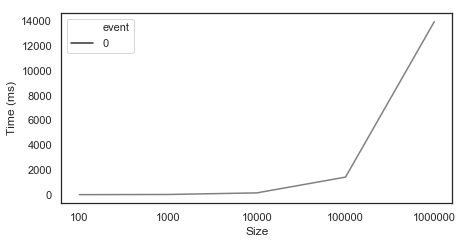
\includegraphics[width=0.4\textwidth]{pictures/introduction/timesize.png}
%	\vspace{-5mm}
%	\caption{The latency time for generating line-based visualization at each datasize.}
%	\vspace{-5mm}
%	\label{fig:rendering_time}
%\end{figure}




%The major challenges to design visual quality guaranteed sampling method are:
%(I) how to define visual quality theoretically? (II) how to guarantee the quality of the sampling-based visualization result?
%\TB{In this work, we study how to reduce the rendering time and preserve the visual quality for the large-scale trajectory visualization.}
%We extend the motivation of visualization-aware sampling to trajectory dataset and propose a novel sampling strategy, \textbf{v}isualization \textbf{a}ware \textbf{t}rajectory \textbf{s}ampling(VATS), that produces high-visual-quality line-based trajectory visualization at different zooming resolutions.
%%\QM{In this paper, we first proposed the visual fidelity loss function which effectively evaluates the visual loss of the sampling method. Then we minimize the loss function by transforming this problem to an optimization problem. Several solutions for efficiently solving the optimization problem are discussed.}
%We first format visual quality by defining the loss function between the visualization results of the whole dataset and sampled dataset.
%With the loss function, we analyze the hardness of the problem, and devise a visual quality guaranteed sampling algorithm for it.
%Figure~\ref{fig:compare} depicts an comparison among the ground truth,  uniform random sampling and our proposed method.
%With the same sampling set size($1\%$), the proposed method generates a higher-fidelity visualization and support the multi-resolution very well.
%At last, color encoding are applied to enhance the distribution of trajectories.
%
%\begin{figure}[t]
%	\centering
%	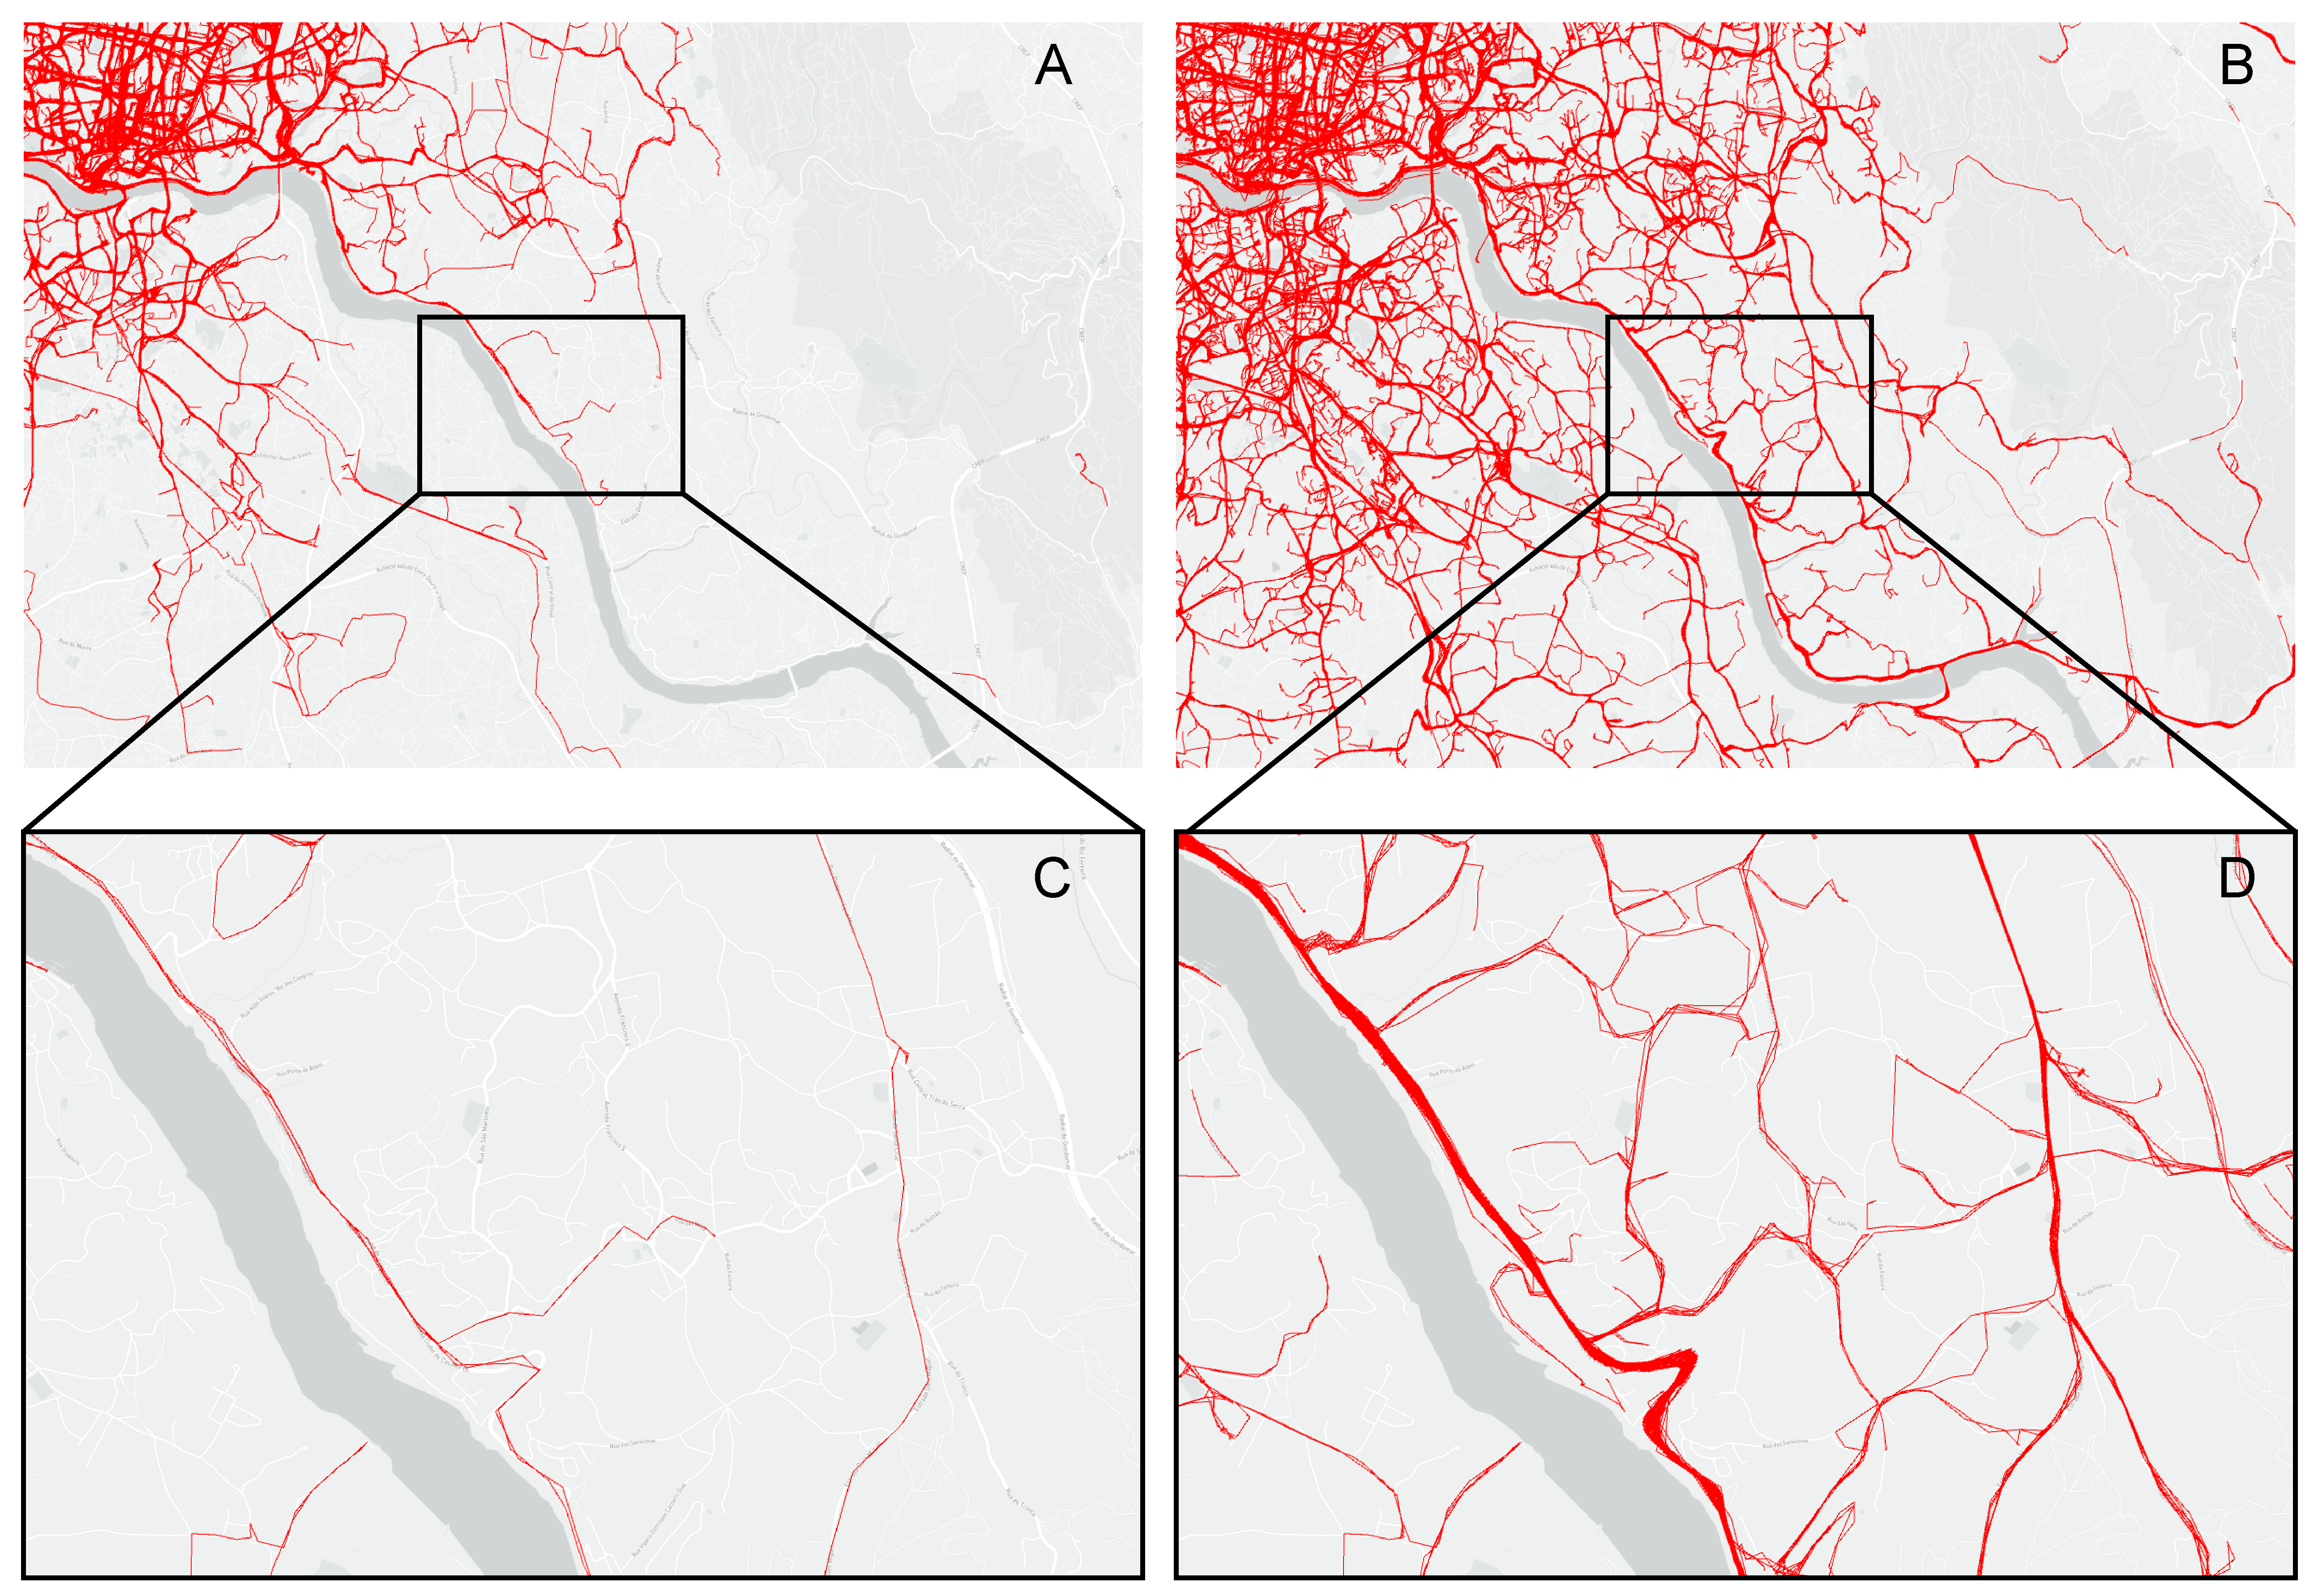
\includegraphics[width=0.44\textwidth]{pictures/introduction/effectiveness.pdf}
%	\vspace{-3mm}
%	\caption{Trajectory sampling generated by uniform random sampling(A,C) and VQGTS(B,D) at same sampling rate. In both high-level(A,B) and low level(C,D) view, our approach preserved more detail information about the trajectories especially for the sparse regions.}
%	\vspace{-5mm}
%	\label{fig:compare}
%\end{figure}
%

%
%
The remainder of this paper is organized as follows.
Section~\ref{sec:rel} discusses the related work.
Section~\ref{sec:pro} formulates our problem and analyze its hardness.
Section~\ref{sec:sol} provides an approximate solution for it, together with a suite of optimization techniques.
Section~\ref{sec:aa} proposes an advanced solution for our problem.
Section~\ref{sec:exp} elaborates our extensive experimental studies and our findings in detail.
Section~\ref{sec:con} concludes this work and highlights the promising future directions.
